%ページ番号消す
\pagestyle{empty}

%レイアウト確認
%\usepackage{layout}

\newif\ifjapanese
\japanesetrue % 論文全体を日本語で書く(英語で書くならコメントアウト)
\ifjapanese
	\documentclass[10pt]{jreport}
	\renewcommand{\bibname}{参考文献}
	\newcommand{\acknowledgmentname}{謝辞}
\else
	\documentclass[10pt]{report}
	\newcommand{\acknowledgmentname}{Acknowledgment}
\fi

\usepackage{ascmac}
\usepackage{here}				%図を強制的に出力する
\usepackage{amsmath}			%枠組み・数式用パッケージ
\usepackage{amssymb}			%数式用パッケージ
\usepackage{multirow}			%段組みのためのパッケージ
\usepackage[dvipdfmx]{graphicx} %PDFへのタイプセットのための関数
\usepackage{mathptmx}			%欧文と数式フォントをAdobe Timesに変更
%\usepackage{mediabb}			%貼り込むPDFのxBBファイルを自動生成
\usepackage{exscale}			%大型演算子のスケーリングもしてくれる。
\usepackage{longtable}			%ページをまたぐ表を、きれいに表示
\usepackage{dcolumn}			%表中で小数点揃えをしてくれる。
\usepackage[a4paper]{geometry}	%余白を1ページだけ調整
\usepackage{style/fancyhdr}		%ヘッダーフッターの調整
\usepackage{caption}			%キャプションの設定
%\usepackage{listings,jlisting}	%同梱「jlisteing」読み込み
								% プログラムソースコードを表示する。
%usepackage[multi,deluxe,bold]{otf}	%OTFフォントの使用(別途mapで設定したものになる)
\usepackage{lscape}              %用紙を横向きにレイアウト
%\usepackage[top=5mm, hmargin=10mm, bottom=25mm]{geometry}
%--------------------------------------------------------------------
\usepackage{style/repo-format}   %同梱の「repo-format.sty」を読込
\usepackage{style/aco-index}     %同梱の「aco-index.sty」を読込
\usepackage{style/roman_math}    %同梱の「roman_math.sty」を読込(ローマ数字)

\begin{document}
\tableofcontents
\pagenumbering{arabic}
\chapter{序論}
\thispagestyle{fancy}
\nobreak
\section{研究背景と目的}
本研究は「オーディトリウムの“底”で演奏を聴く」という旧態依然とした鑑賞形態並びにそれに基づく決定論的設計法に対し、建築音響学の観点から新たな息吹を吹き込むことで、次世代の建築を設計するための礎を築こうとするものである。

\subsection{2階バルコニー最前列席の音響的評価}
この世に存在する全てのオーディトリウムはいずれも室固有の響きを持っており、それは室を構成する形と内装条件によって決定づけられる。一般的な音響設計では、どの客席においても一様な反射音が到達するよう計画される。
ここで、収容人数や舞台へ向けての視野を確保する観点から、オーディトリウムにバルコニー席を設けることが多々ある。このとき、バルコニー先端部は前方に客席がなく、ホール空間へ張り出した特異な場となる。
\\ さて、2階バルコニー最前列の座席は、音響的に高い評価を得ることが多い$^{\text{\cite{01-1}}}$。これは、ホール空間が有する吸音力の大半(500Hzで7割程度)$^{\text{\cite{01-2}}}$を受け持っている1階客席床面(椅子+聴衆の吸音力)から相対的に離れた場所に位置するため、エネルギ減衰の少ない有効な直接音や反射音を得やすいことに起因すると定性的に推察されている(\textgt{図}\ref{fig:2階バルコニー最前列席の音場})。
\\
\\
\begin{figure}[h]
    \centering
    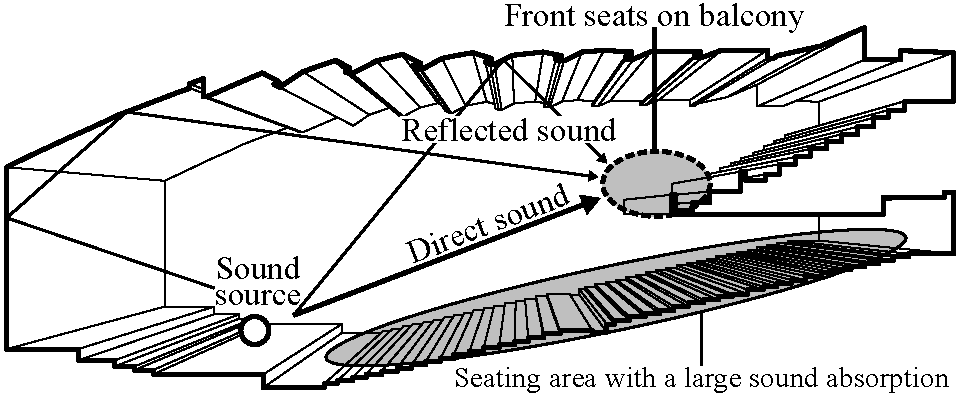
\includegraphics[keepaspectratio,scale=0.8]{01_att/second_balcony.pdf}
    \caption{\hspace{1mm}2階バルコニー最前列席の音場}
    \label{fig:2階バルコニー最前列席の音場}
\end{figure}

%-------------------------------------------------------------
\newpage
\subsection{評価対象領域の拡張}
美しい響きを生み出すにあたり、室容積は人間を収容するには冗長な大きさを要する。規模により異なるものの、室容積から算出されるホールの天井高はおおよそ10$\sim$20mである。ホール空間は人が鑑賞可能なエリアを断面方向含め無数に拡張できるというポテンシャルを秘めているにも関わらず、オーディトリウムの底で鑑賞をするという様式は依然として変わっていない。
\\ 建築音響学が体系化した1900年以後$^{\text{\cite{01-3}}}$、ホールの音響性能について種々研究が行われているものの、音場測定や解析シミュレーションによる音場の評価は、当然のことながら、建築的に確定された客席床面(床面上高さ1$\sim$2m)における面的評価に留まっており、ホール空間全体を評価対象とした設計研究は皆無である。本研究では、前節で述べた知見を踏まえ、評価対象領域を3次元的に拡張した評価を試みる(\textgt{図}\ref{fig:評価対象領域の拡張})。
\\
\begin{figure}[h]
    \centering
    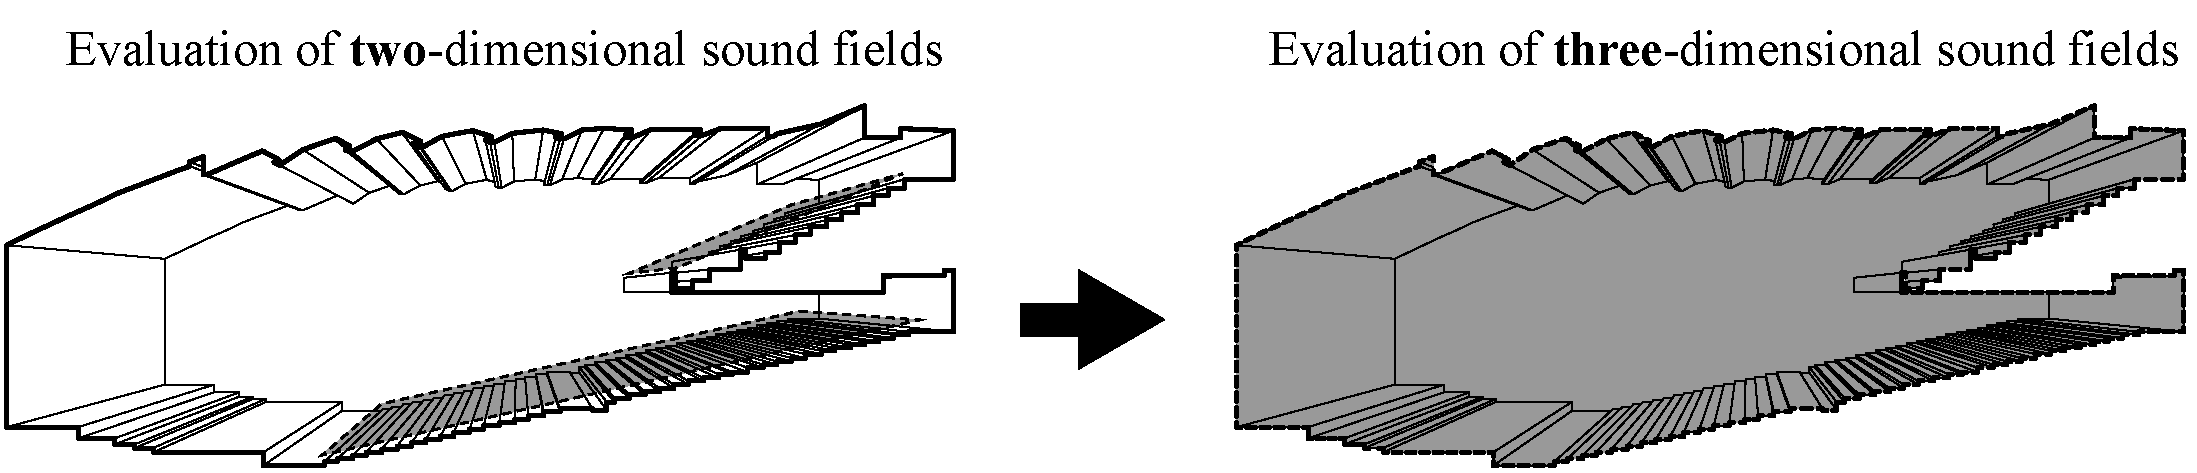
\includegraphics[keepaspectratio,scale=0.41]{01_att/evaluate_area.pdf}
    \caption{\hspace{1mm}評価対象領域の拡張}
    \label{fig:評価対象領域の拡張}
\end{figure}

\subsection{研究目的}
本研究は、コンサートホール音場の評価対象領域を、吸音力の大きな座席面近傍音場から3次元的に拡張し、座席面遠方音場(\textgt{図}\ref{fig:座席面遠方音場})の音響物理特性を明らかにすることにより、従来の面的評価並びにそれに基づく決定論的設計法に新たな可能性を見出すことを目的とするものである。
\\
\begin{figure}[h]
    \centering
    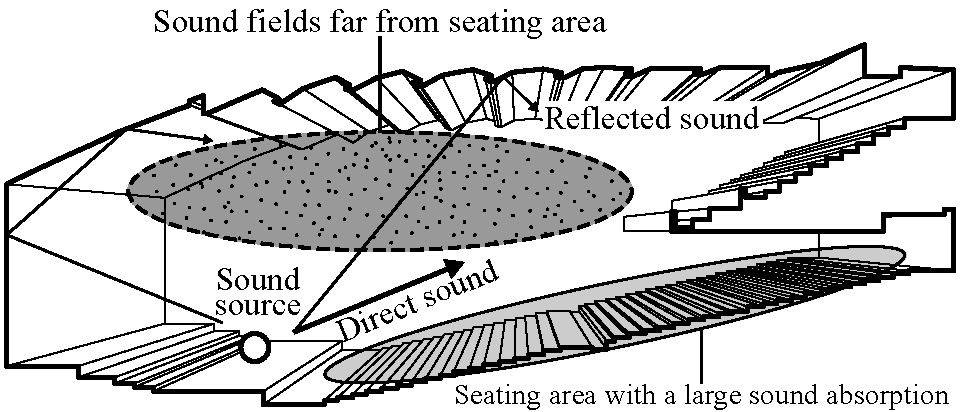
\includegraphics[keepaspectratio,scale=0.8]{01_att/zasekimen_enpo_English.pdf}
    \caption{\hspace{1mm}座席面遠方音場}
    \label{fig:座席面遠方音場}
\end{figure}

%-------------------------------------------------------------
\newpage
\section{既往の研究と本論の位置づけ}
\subsection{音環境の心理評価システム}
物理的特性と聴覚的効果との対応を考える必要があることを説明する
\\→本論文は物理的特性をとりあげた研究であること(聴覚的効果との対応は含まない)を言及する。

\subsection{室内音響物理指標}
4つの要素感覚とそれに対応すると提案されている物理量について説明する。

\subsection{フライングバルコニーを有するホールの事例}
Philharmonie de Parisを例にフライングバルコニーの紹介、本研究のテーマに近いホールがあることを示し、本テーマは突拍子もないことではないことを示す。

\section{論文構成}
本論文は、以下に示す全7章で構成される。
\\ 第1章では前節までに本研究の背景と目的、関連する既往研究の概要、本論の位置づけについて述べた。本節では、論文の構成について述べている。
\\ 第2章では、研究手法である幾何音響解析の概要、解析条件並びに解析モデルについて述べる。
\\ 第3章では、解析で得られたデータから残響特性の観点から音場評価を行う。
\\ 第4章では、時間エネルギ特性の観点から音場評価を行う。
\\ 第5章では、反射音方向分布特性の観点から距離減衰特性及び方向別エネルギ率の観点から音場評価を行う。
\\ 第6章では、これまでの研究結果を踏まえ、ホール形状の設計例を提示する。
\\ 最後の第7章では、本論文の結論を述べる。

\chapter{空間全体を対象とした幾何音響解析}
\section{幾何音響解析手法について}
幾何音響解析手法とは、音の波動としての性質を無視して、その伝搬を幾何的に取り扱う手法のことである$^{\text{\cite{02-5}}}$。非常に直感的で理解しやすい方法であり、あまり多くの計算機資源を必要とせず、計算時間も波動音響解析手法と比べ短いため、大規模空間を扱う際の現実的手法として広く用いられている。厳密な予測が必要となる詳細設計の段階では音響縮尺模型実験や波動音響解析に頼らざるを得ないが、基本計画段階における検討や初期反射音構造の予測等に対しては大変有用であると考えられている。
幾何音響学に基づいた代表的なコンピュータシミュレーション手法として、音線法と鏡像法が挙げられる(\textgt{図}\ref{fig:音線法と鏡像法})。
\\ 音線法(Ray-tracing method)とは、音源から等立体間隔で多数の音線を出すことで、反射伝搬経路を追跡計算する手法であり、距離減衰は音線間の広がり(音線の密度)によって考慮される。なお、有限の間隔で放射された音線が丁度受音点を通過することは極めて稀なため、有限の大きさを持つ受音領域を設けることが一般的である。しかしながら、受音点が領域を持つゆえに同一経路の反射音が重複したり、現実にはない反射経路を抽出したり等の計算誤差が生じる。この問題を解決するため、複数のアルゴリズムが考案されている$^{\text{\cite{02-6}}}$。
\\ 鏡像法(Image source method)は周壁各面における音源の鏡像を幾何学的に求め、各鏡像から受音点までの経路を求める手法である。距離減衰と通った反射面の吸音率からインパルス応答を近似的に求めることができるが、反射次数の増加とともに鏡像の数が指数関数的に増加するため、高次の反射音まで求めることは困難である$^{\text{\cite{02-5}}}$。
\\ 音線法と鏡像法のいずれも、初期反射音の検討に対して非常に有用であると考えられるが、拡散反射を考慮できない幾何音響シミュレーションのみでは、反射回数が増加するに従い、現実の音場との誤差が大きくなってしまう。そこで近年では乱反射率(Scattering coefficient)などの導入により、室内音場の長時間のインパルス応答を求めようとする試みがある。

\begin{figure}[H]
    \centering
    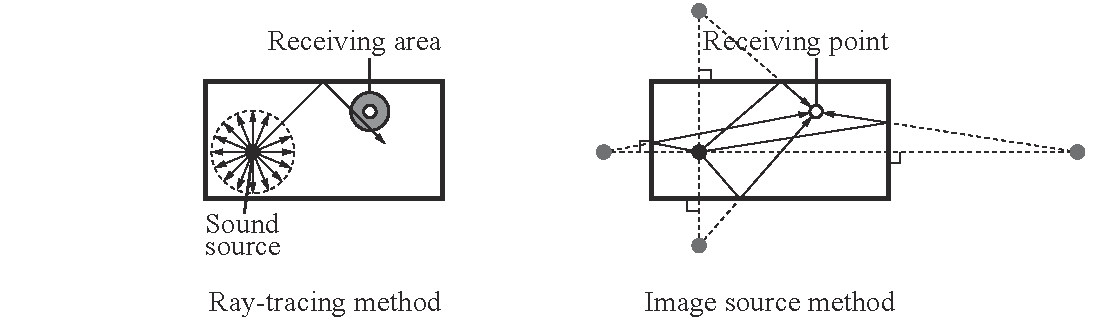
\includegraphics[keepaspectratio,scale=0.8]{02_att/kikaonkyo.pdf}
    \caption{\hspace{1mm}音線法と鏡像法の概念図}
    \label{fig:音線法と鏡像法}
\end{figure}

\section{解析条件}
本研究で用いる幾何音響解析ソフトには3つの解析タイプ(Audio area mapping, Early part detailed, Full detailed calculation)があり、それぞれ音線法、鏡像法、Randomized Tail-corrected Cone-tracing(RTC)の解析手法が用いられている。
RTCとは音線の先に円の有限領域をもたせるCone-tracingと標準的な音線法及び鏡像法をハイブリッドした解析手法である。
\\ 本研究では、これらのうち後期音までのインパルス応答を算出するFull detailed calculationと、方向情報を含んだ初期音のインパルス応答を算出するEarly part detailedの2つの解析タイプを使用した。それぞれの解析タイプで出力されるインパルス応答を\textgt{図}\ref{fig:Full_IR}と\textgt{図}\ref{fig:Early_IR}に、解析条件を\textgt{表}\ref{Full_set}及び\textgt{表}\ref{Early_set}に示す。
\\ また、音速と空気吸収は\textgt{式}\ref{eq:speed_of_sound}と\textgt{式}\ref{eq:air_absorption}により設定される。

\begin{equation}
 \label{eq:speed_of_sound}
c = 331.4\sqrt{1+\frac{\theta}{273}}
\end{equation}

\begin{equation}
 \label{eq:air_absorption}
m_b = \mathrm{from \; ISO \; 9613.1^{\text{\cite{organizacion1993iso}}} \; based \; on \; \theta, \; f_b, \; and \; \phi}
\end{equation}



気温\(20^\circ\)、相対湿度50\%、空気の比重を1.2kg/m$^3$に設定した。
この条件により、音速と空気吸収が定まる。
\subsubsection{Early part detailed ISM}

\subsubsection{Full detailed calculation}

\section{解析モデル}
解析モデルは収容人員1,500人程度のコンサートホールを想定し、平面形状が矩形のモデル(TypeA)と扇形のモデル(TypeB)の2種類の空間モデルを対象とした。両モデルとも舞台高さを1m、奥行きを10mに統一した。
\\ 観測点は客席床面上と上部空間の音場性能を比較するために2m\(\times\)2m\(\times\)2mの格子状に(A)矩形モデルで840点、(B)扇形モデルで712点設けた。
また、音線が音源方向から到来したときに反射音到来角度が\(0^\circ\)になるよう、観測点の座標系を設定した。
音源は無指向性音源を舞台中央に高さ1.5mとした。両ホールの音響諸元を\textgt{表}\ref{解析モデルの音響諸元}に示す。
%%%%%%%%%%%%%%%%%%%
\begin{table}[htbp]
\centering
\caption{解析モデルの音響諸元}
\label{解析モデルの音響諸元}
\begin{tabular}{lccccc}
\Hline
\multicolumn{1}{c}{Type} & \textit{V}{[}m$^3${]} & \textit{V}/\textit{S}{[}m{]} & \textit{RT}$^{*1}${[}s{]} &$\bar{\alpha}$& N$^{*2}$ \\ \hline
(A)Rectanglular & 15,268 & 3.8 & 2.2 & 0.24 & 840 \\
(B)Fan-shape & 15,329 & 3.8 & 2.2 & 0.24 & 712 \\ \Hline
\multicolumn{6}{l}{$^{*1}$ : calculated with Eyring-Knudsen formula (500Hz)} \\
\multicolumn{4}{l}{$^{*2}$ : N indicates the number of receiving points}
\end{tabular}
\end{table}
%%%%%%%%%%%%%%%%%%%

\subsection{形状の設計}
現存するホールを参考$^{\text{\cite{02-1}}}$に(A)矩形モデル及び(B)扇形モデルの設計を行った。
両ホールの断面図及び平面図を\textgt{図}\ref{fig:(A)矩形モデル及び(B)扇形モデルの断面図}、\textgt{図}\ref{fig:(A)矩形モデル平面図}、\textgt{図}\ref{fig:(A)矩形モデル平面図}に示す。

\subsection{吸音率の設定}
室の内装面は客席床と後壁を吸音性、その他の面を反射性とし、両ホールの残響時間が等しくなるように現実的な吸音率(250$\sim$2kHz)$^{\text{\cite{01-3}\cite{02-1}\cite{02-2}}}$を設定した。客席床の吸音率については国内の標準的な1席(人+モケット張り椅子)の吸音力$^{\text{\cite{02-4}}}$を1席あたりの床面積(=0.6m$^2$)で除した値(\textgt{表}\ref{客席面の吸音率})を用いた。解析モデルに用いた吸音率を\textgt{表}\ref{解析モデルの吸音率}に示す。

%%%%%%%%%%%%%%%%%%%
\begin{table}[htbp]
\begin{center}
\caption{客席面の(a)吸音力と(b)吸音率}
\label{客席面の吸音率}
\begin{tabular}{llcccccc}
\Hline
&&\multicolumn{6}{c}{Frequency{[}Hz{]}}\\\cline{3-8}
&&125&250&500&1k&2k&4k\\\hline
(a)&\begin{tabular}[c]{@{}l@{}}Sound absorption of a seat \\(human and moquette-clad chair) \end{tabular}&0.23&0.32&0.40&0.43&0.43&0.41\\\hline
(b)&\begin{tabular}[c]{@{}l@{}}Sound absorption coefficient \\equivalent to (a)\end{tabular}&0.38&0.53&0.67&0.72&0.72&0.68\\\Hline
\end{tabular}
\end{center}
\end{table}
%%%%%%%%%%%%%%%%%%%

%%%%%%%%%%%%%%%%%%%
\begin{table}[H]
\centering
\caption{解析モデルの吸音率}
\label{解析モデルの吸音率}
\resizebox{\textwidth}{!}{%
\begin{tabular}{llcccccc}
\Hline
                         &                                           & \multicolumn{6}{c}{Frequency{[}Hz{]}}   \\ \cline{3-8} 
\multicolumn{1}{c}{Site} & \multicolumn{1}{c}{Material}              & 125  & 250  & 500  & 1k   & 2k   & 4k   \\ \hline
Ceiling \_ main floor    & Plaster board (12mm) with large air space & 0.25 & 0.15 & 0.10 & 0.08 & 0.06 & 0.05 \\
Ceiling \_ stage         & Acoustic reflector                        & 0.15 & 0.15 & 0.10 & 0.08 & 0.07 & 0.06 \\
Floor \_ main floor      & Human and moquette-clad chair             & 0.38 & 0.53 & 0.67 & 0.72 & 0.72 & 0.68 \\
Floor \_ stage           & Floor joist of stage (45mm)               & 0.15 & 0.10 & 0.08 & 0.07 & 0.05 & 0.05 \\
Side wall \_ main floor  & Concrete                                  & 0.01 & 0.02 & 0.02 & 0.03 & 0.03 & 0.03 \\
Rear wall \_ main floor  & Glass wool (25mm) with large air space    & 0.55 & 0.80 & 0.75 & 0.48 & 0.33 & 0.15 \\
Wall \_ stage            & Acoustic reflector                        & 0.15 & 0.15 & 0.10 & 0.08 & 0.07 & 0.06 \\ \Hline
\end{tabular}%
}
\end{table}
%%%%%%%%%%%%%%%%%%%

\subsection{乱反射率の設定}
乱反射率(Scattering coefficient)はISO17497-1$^{\text{\cite{iso2004acoustics}}}$の中で壁面の全反射エネルギーに対する鏡面反射成分以外のエネルギーの割合として定義され、\textgt{式}\ref{eq:scatter}で表される。ここで$E_{total}$は全反射エネルギー、$E_{spec}$は鏡面反射エネルギーである。

\begin{equation}
 \label{eq:scatter}
s_{\theta}=1-\frac{E_{spec}}{E_{total}}
\end{equation}
\\ 解析では、周波数に応じて座席部に0.3$\sim$0.7を、それ以外の面に0.1を与えた$^{\text{\cite{02-3}}}$。
解析モデルに用いた乱反射率を\textgt{表}\ref{解析モデルの乱反射率}に示す。\\
 また、壁面隅角部における音の散乱(端部散乱)を考慮した乱反射率を与える研究$^{\text{\cite{02-7}}}$が進められている。
壁面端部から$\lambda$/8分の面積を1、それ以外の面積を0として面積平均した乱反射率を吸音面の接合面に与えたときに実測との対応が良くなることが既往の研究$^{\text{\cite{02-8}}}$から明らかになっているが、これは本研究で使用する幾何音響解析ソフトの端部散乱を考慮した乱反射率(壁面端部から$\lambda$/4分の面積を0.5、それ以外の面積を0として面積平均したもの(\textgt{式}\ref{eq:付加乱反射率計算式}、\textgt{図}\ref{fig:壁面端部}))に近似する。
解析モデルにおいて端部散乱を考慮した面を\textgt{表}\ref{端部散乱を適用する面}に示す。
%%%%%%%%%%%%%%%%%%%
\begin{table}[htbp]
\centering
\caption{解析モデルの乱反射率}
\label{解析モデルの乱反射率}
\resizebox{\textwidth}{!}{%
\begin{tabular}{llcccccc}
\Hline
&& \multicolumn{6}{c}{Frequency{[}Hz{]}}   \\ \cline{3-8} 
\multicolumn{1}{c}{Site} & \multicolumn{1}{c}{Material}              & 125  & 250  & 500  & 1k   & 2k   & 4k   \\ \hline
Ceiling \_ main floor    & Plaster board (12mm) with large air space & 0.10 & 0.10 & 0.10 & 0.10 & 0.10 & 0.10 \\
Ceiling \_ stage         & Acoustic reflector                        & 0.10 & 0.10 & 0.10 & 0.10 & 0.10 & 0.10 \\
Floor \_ main floor      & Human and moquette-clad chair             & 0.30 & 0.40 & 0.50 & 0.60 & 0.70 & 0.80 \\
Floor \_ stage           & Floor joist of stage (45mm)               & 0.10 & 0.10 & 0.10 & 0.10 & 0.10 & 0.10 \\
Side wall \_ main floor  & Concrete                                  & 0.10 & 0.10 & 0.10 & 0.10 & 0.10 & 0.10 \\
Rear wall \_ main floor  & Glass wool (25mm) with large air space    & 0.10 & 0.10 & 0.10 & 0.10 & 0.10 & 0.10 \\
Wall \_ stage            & Acoustic reflector                        & 0.10 & 0.10 & 0.10 & 0.10 & 0.10 & 0.10 \\ \Hline
\end{tabular}%
}
\end{table}
%%%%%%%%%%%%%%%%%%%

\pagebreak
\begin{equation}
 \label{eq:付加乱反射率計算式}
 s_{\scalebox{0.5}{effective}} = s_{\scalebox{0.5}{surface}} + \frac{s_{\scalebox{0.5}{edge}}
 S_{\scalebox{0.5}{edge}}}{S_{\scalebox{0.5}{surface}}}\\
\end{equation}
\hspace{3cm}$s_{\scalebox{0.5}{edge}} = 0.5$\\
\hspace{3cm}$s_{\scalebox{0.5}{surface}}$ : The normal surface scattering coefficient\\
\hspace{3cm}$S_{\scalebox{0.5}{edge}}$ : The area of an edge quarter of a wavelength wide\\
\hspace{3cm}$S_{\scalebox{0.5}{surface}}$ : The complete plane or sub-plane area\\


\begin{figure}[H]
    \centering
    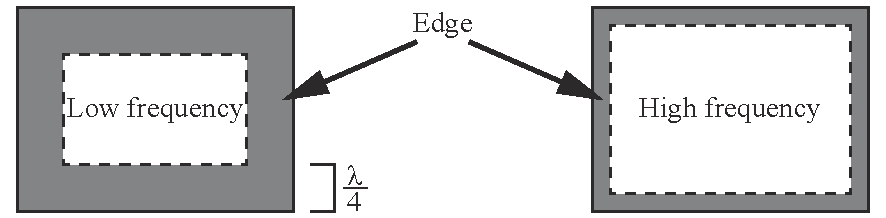
\includegraphics[keepaspectratio,scale=0.8]{02_att/edge.pdf}
    \caption{\hspace{1mm}壁面端部から$\lambda$/4分の面積}
    \label{fig:壁面端部}
\end{figure}

%%%%%%%%%%%%%%%%%%%
\begin{table}[H]
\centering
\caption{端部散乱を適用する面}
\label{端部散乱を適用する面}
\begin{tabular}{llc}
\Hline
\multicolumn{1}{c}{Site} & \multicolumn{1}{c}{Type} & Apply edge diffusion to surface \\ \hline
Ceiling \_ main floor    & Reflective               & *                               \\
Ceiling \_ stage         & Reflective               & *                               \\
Floor \_ main floor      & Absorptive               &                                 \\
Floor \_ stage           & Reflective               & *                               \\
Side wall \_ main floor  & Reflective               & *                               \\
Rear wall \_ main floor  & Absorptive               &                                 \\
Wall \_ stage            & Reflective               & *                               \\ \Hline
\end{tabular}
\end{table}
%%%%%%%%%%%%%%%%%%%

\chapter{残響特性の評価}
\section{分析手法}
\subsection{一元配置分散分析}
残響時間は正規分布に従うため、一元配置分散分析を行う。
\subsection{ノンパラメトリック分散分析}
EDTを観測高さごとに比較するため、ノンパラメトリック分散分析を行う。
\section{観測高さの違いと残響特性の分析}


\chapter{音響エネルギ分布特性}

一元配置分散分析(対応あり)の結果を\tabref{ichigen}に示す。
$EDT$を除く全ての指標値で有意な差が認められた。
次にHolmの多重比較を行った結果を\tabref{Gtaju}$\sim$\tabref{Ttaju}に示す。

\begin{table}[H]
\centering
\caption{The result of one-way analysis of variance}
\label{tab:ichigen}
\begin{tabular}{cccccccc}
\Hline
\begin{tabular}[c]{@{}c@{}}Acoustic\\ parameter\end{tabular} & \textit{G} & \textit{EDT} & $C_{80}$ & $D_{50}$ & \textit{LF} & \textit{IACC} & $T_{30}$ \\ \hline
judge & ** & n.s. & * & ** & ** & ** & ** \\ \Hline
\multicolumn{8}{l}{**:$p$\textless{}0.01, *:$p$\textless{}0.05}
\end{tabular}
\end{table}

\begin{table}[H]
\centering
\caption{$G$ of the test results}
\label{tab:Gtaju}
\begin{tabular}{ccccccccc}
\Hline
 & 1.2 & 2.0 & 4.0 & 6.0 & 8.0 & 10.0 & 12.0 & 14.0 \\ \hline
1.2 &  & n.s. & n.s. & n.s. & n.s. & n.s. & n.s. & n.s. \\
2.0 &  &  & n.s. & n.s. & n.s. & n.s. & * & ** \\
4.0 &  &  &  & n.s. & n.s. & n.s. & ** & ** \\
6.0 &  &  &  &  & n.s. & n.s. & n.s. & n.s. \\
8.0 &  &  &  &  &  & n.s. & n.s. & n.s. \\
10.0 &  &  &  &  &  &  & n.s. & n.s. \\
12.0 &  &  &  &  &  &  &  & n.s. \\
14.0 &  &  &  &  &  &  &  &  \\ \Hline
\end{tabular}
\end{table}

\begin{table}[H]
\centering
\caption{$D_{50}$ of the test results}
\label{tab:Dtaju}
\begin{tabular}{ccccccccc}
\Hline
 & 1.2 & 2.0 & 4.0 & 6.0 & 8.0 & 10.0 & 12.0 & 14.0 \\ \hline
1.2 &  & n.s. & n.s. & n.s. & n.s. & n.s. & n.s. & n.s. \\
2.0 &  &  & n.s. & n.s. & n.s. & n.s. & n.s. & n.s. \\
4.0 &  &  &  & n.s. & n.s. & n.s. & n.s. & n.s. \\
6.0 &  &  &  &  & n.s. & n.s. & n.s. & n.s. \\
8.0 &  &  &  &  &  & n.s. & n.s. & * \\
10.0 &  &  &  &  &  &  & n.s. & * \\
12.0 &  &  &  &  &  &  &  & n.s. \\
14.0 &  &  &  &  &  &  &  &  \\ \Hline
\end{tabular}
\end{table}

\begin{table}[H]
\centering
\caption{$LF$ of the test results}
\label{tab:LFtaju}
\begin{tabular}{ccccccccc}
\Hline
 & 1.2 & 2.0 & 4.0 & 6.0 & 8.0 & 10.0 & 12.0 & 14.0 \\ \hline
1.2 &  & n.s. & n.s. & n.s. & * & ** & ** & ** \\
2.0 &  &  & n.s. & n.s. & * & ** & ** & ** \\
4.0 &  &  &  & n.s. & * & ** & ** & ** \\
6.0 &  &  &  &  & n.s. & * & ** & ** \\
8.0 &  &  &  &  &  & n.s. & * & ** \\
10.0 &  &  &  &  &  &  & n.s. & n.s. \\
12.0 &  &  &  &  &  &  &  & n.s. \\
14.0 &  &  &  &  &  &  &  &  \\ \Hline
\end{tabular}
\end{table}

\begin{table}[H]
\centering
\caption{$IACC$ of the test results}
\label{tab:IACCtaju}
\begin{tabular}{ccccccccc}
\Hline
 & 1.2 & 2.0 & 4.0 & 6.0 & 8.0 & 10.0 & 12.0 & 14.0 \\ \hline
1.2 &  & n.s. & n.s. & n.s. & n.s. & ** & ** & ** \\
2.0 &  &  & n.s. & n.s. & n.s. & n.s. & ** & ** \\
4.0 &  &  &  & n.s. & n.s. & n.s. & ** & ** \\
6.0 &  &  &  &  & n.s. & n.s. & ** & ** \\
8.0 &  &  &  &  &  & n.s. & * & ** \\
10.0 &  &  &  &  &  &  & n.s. & ** \\
12.0 &  &  &  &  &  &  &  & n.s. \\
14.0 &  &  &  &  &  &  &  &  \\ \Hline
\end{tabular}
\end{table}

\begin{table}[H]
\centering
\caption{$T_{30}$ of the test results}
\label{tab:Ttaju}
\begin{tabular}{ccccccccc}
\Hline
 & 1.2 & 2.0 & 4.0 & 6.0 & 8.0 & 10.0 & 12.0 & 14.0 \\ \hline
1.2 &  & ** & n.s. & ** & ** & ** & ** & ** \\
2.0 &  &  & n.s. & ** & ** & ** & ** & ** \\
4.0 &  &  &  & ** & ** & ** & ** & ** \\
6.0 &  &  &  &  & ** & n.s. & n.s. & n.s. \\
8.0 &  &  &  &  &  & n.s. & n.s. & ** \\
10.0 &  &  &  &  &  &  & n.s. & * \\
12.0 &  &  &  &  &  &  &  & * \\
14.0 &  &  &  &  &  &  &  &  \\ \Hline
\end{tabular}
\end{table}

\pagebreak
残響エネルギ特性に関する指標$T_{30}$や反射音の方向情報より算出される指標$LF,IACC$では観測高さによる平均値の違いが多く見られた一方、時間エネルギ特性に関する指標$D_{50},C_{80}$及び音圧レベル特性に関する指標$G$では、観測高さによる平均値の違いはあまりみられなかった。

ここで、$G$及び$G_{early}$,$G_{late}$,$C_{80}$と音源-観測点間距離$r$[m]の関係をBarronによる理論値と共に\figref{G_Barron},\figref{Ge_Barron},\figref{Gl_Barron},\figref{C_Barron}に示す。観測高さ$H$=14.0の観測点は音源から遠い位置に分布しているため、いずれの指標値も一定の範囲内に集中している。このことから、座席面遠方音場ではその観測高さ内でとる値のバラつきが小さくなる様子が伺える。

\begin{figure}[H]
    \centering
    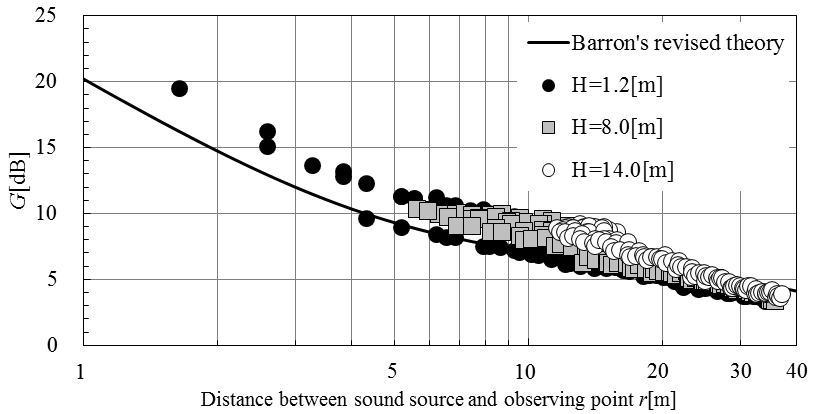
\includegraphics[keepaspectratio,scale=1]{04_att/G_Barron.png}
    \caption{\hspace{1mm}$G$ vs distance between sound source and observing point}
    \label{fig:G_Barron}
\end{figure}

\begin{figure}[H]
    \centering
    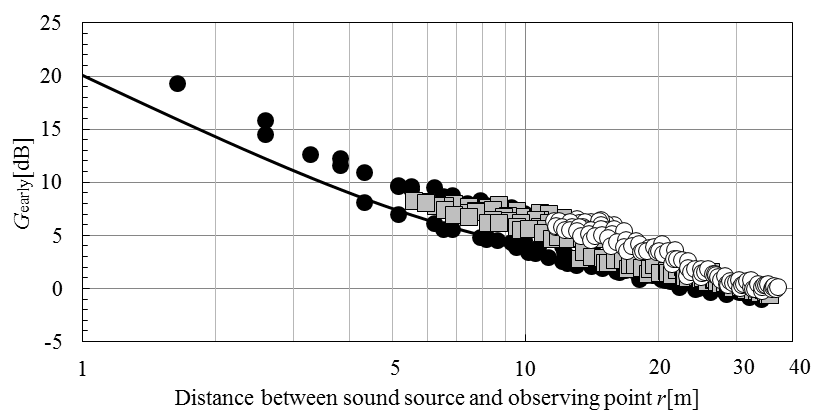
\includegraphics[keepaspectratio,scale=1]{04_att/Ge_Barron.png}
    \caption{\hspace{1mm}$G_{early}$ vs distance between sound source and observing point}
    \label{fig:Ge_Barron}
\end{figure}

\begin{figure}[H]
    \centering
    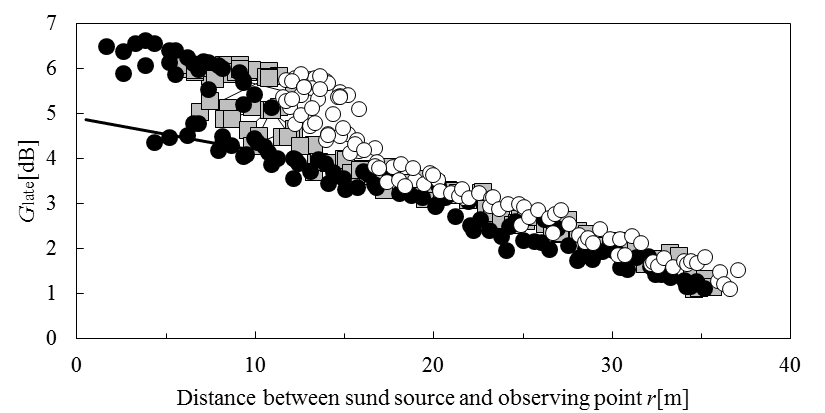
\includegraphics[keepaspectratio,scale=1]{04_att/Gl_Barron.png}
    \caption{\hspace{1mm}$G_{late}$ vs distance between sound source and observing point}
    \label{fig:Gl_Barron}
\end{figure}

\begin{figure}[H]
    \centering
    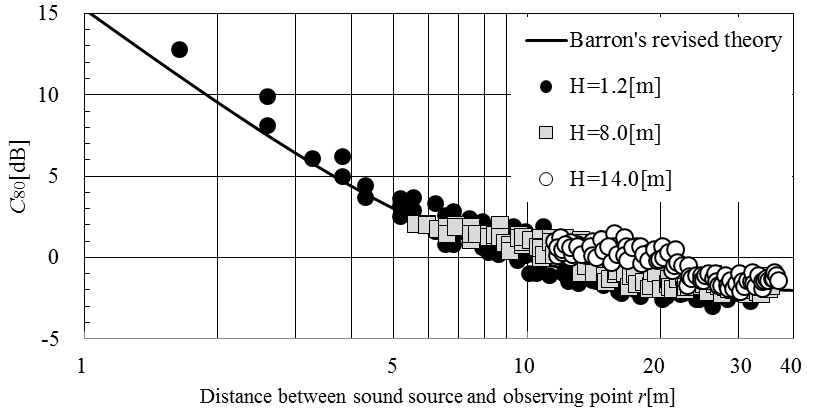
\includegraphics[keepaspectratio,scale=1]{04_att/C_Barron.png}
    \caption{\hspace{1mm}$C_{80}$ vs distance between sound source and observing point}
    \label{fig:C_Barron}
\end{figure}

そこで、音響エネルギ分布の一様度を定量的にみるため、各指標値から平均値と標準偏差を観測高さごとに求めた(\figref{G},\figref{Ge},\figref{Gl},\figref{C})。観測高さによる平均値の変化幅と標準偏差の変化幅の観点から音響エネルギ分布の一様度について考察を行う。
\\ まず$G$を見てみる。平均値の観測高さによる変化幅は0.4dB(6.6$\sim$7.0dB)とほぼ一定の値を示した一方、標準偏差の観測高さによる変化幅は1.3dB(3.1$\sim$1.8dB)であった。これは$G$の弁別閾($\geq$1dB)を上回るため、有意な差であるといえる。加えて、観測高さが上がるにつれて標準偏差が小さくなる傾向が確認できる。
\\ 次に$G_{early}$を見てみる。平均値の変化幅は0.4dB(3.4$\sim$3.8dB)と大きな変動は見られない。一方、標準偏差の変化幅は2.0dB(2.3$\sim$4.2dB)であり、有意な差が確認できた。$G_{early}$は初期音(直接音+初期反射音)から算出される指標であるため、観測点位置による音響エネルギ分布の違いが顕著であったと考えられる。
\\ $G_{late}$をみてみる。平均値の変化幅は0.2dB(1.4$\sim$1.6dB)とほぼ一定の値であった。また、標準偏差の変化幅についても0.2dB(3.7$\sim$3.9dB)とおおよそ一定の値であった。後期反射音は十分に拡散した反射音であるから観測点位置による偏りがなく、一様に分布するため、観測高さによる差が出なかったと考えられる。
\\ 最後に$C_{80}$についてみてみる。平均値の変化幅は0.4dB(-0.4$\sim$0.0dB)とほぼ一定の値をとるが、標準偏差の変化幅は1.8dB(1.0$\sim$2.8dB)であった。これは、$C_{80}$の弁別域($\geq$1dB)を上回るため、有意な差である。また、$G$と同様に$C_{80}$も観測高さが上がるにつれて標準偏差が小さくなる傾向が見られた。
\\ 以上の分析から、座席面遠方音場では近傍音場に比べ音響エネルギ分布がより一様であることがわかる。

\begin{figure}[htbp]
    \centering
    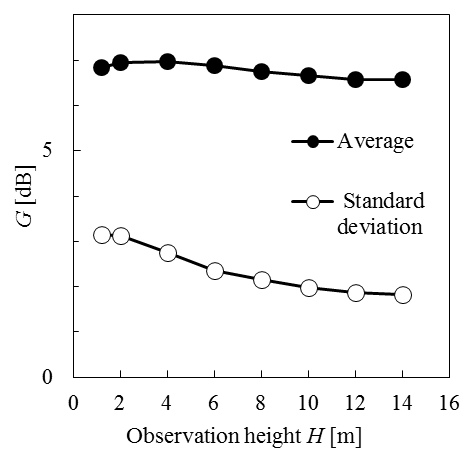
\includegraphics[keepaspectratio,scale=1]{04_att/G.png}
    \caption{\hspace{1mm}Spatial distribution of $G$}
    \label{fig:G}
\end{figure}

\begin{figure}[htbp]
    \centering
    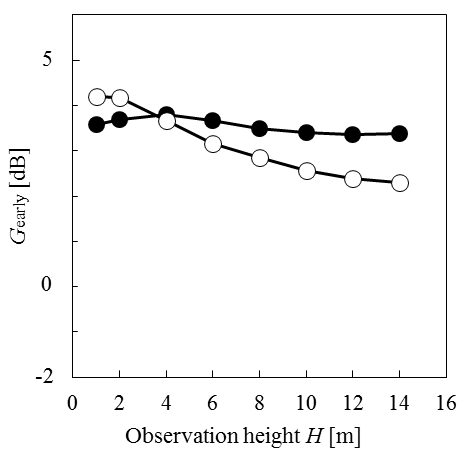
\includegraphics[keepaspectratio,scale=1]{04_att/Ge.png}
    \caption{\hspace{1mm}Spatial distribution of $G_{early}$}
    \label{fig:Ge}
\end{figure}

\begin{figure}[htbp]
    \centering
    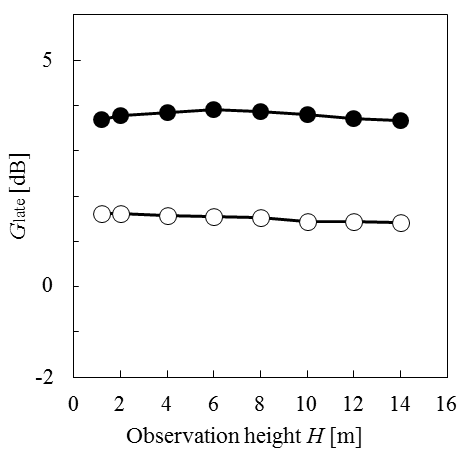
\includegraphics[keepaspectratio,scale=1]{04_att/Gl.png}
    \caption{\hspace{1mm}Spatial distribution of $G_{late}$}
    \label{fig:Gl}
\end{figure}

\begin{figure}[htbp]
    \centering
    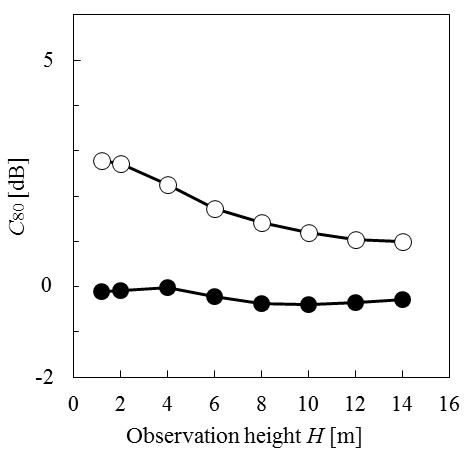
\includegraphics[keepaspectratio,scale=1]{04_att/C.png}
    \caption{\hspace{1mm}Spatial distribution of $C_{80}$}
    \label{fig:C}
\end{figure}

\chapter{拡散性評価}
\section{距離減衰特性}
\subsection{距離減衰特性に関する理論値}
BarronのRevised Theoryを説明。
\subsection{初期音に関する物理量}
GearlyとVGearly,LGearly,GGearlyの算出法を記述。
\subsection{減衰率の算出}
回帰直線の傾きから減衰率[dB/dd]を算出する旨。
\subsection{観測高さの違いと距離減衰特性の分析}
\subsection{客席面吸音率の変化と距離減衰特性の分析}
客席面を吸音性/反射性にしたときに距離減衰特性がどのように変化したかを記述。
\section{方向別エネルギ率}
\subsection{初期音の方向別物理量}
ERv,ERl,ERgの説明。
\subsection{DUIの導入}
\subsection{観測高さの違いと反射音方向分布特性の分析}
\subsection{客席面吸音率の変化と反射音方向分布特性の分析}
\chapter{時間エネルギ特性評価}

\chapter{結論}

%******** 付 属 品 **********************************
\begin{acknowledgment}
\thispagestyle{fancy}
%本論文は筆者が芝浦工業大学工学部建築学科古屋研究室在学中に行った研究をまとめたものです。
この1年間、ご指導ご高配を賜りました芝浦工業大学教授・古屋浩先生に厚くお礼申し上げます。
先生には研究の進め方から物事に取り組む姿勢、資料の表現方法に至るまで終始厳しくも優しい御指導を賜りました。また、研究に関する御指導だけでなく、日頃の研究室活動においても常に温かいご配慮をいただきました。
「工学的に建築を捉える」というテーマに向かって、これまで研究指導して下さいましたことに重ねて御礼申し上げます。
\\ 古屋研究室の先輩である藤田鋭志さん、原彩乃さん、平舘勇馬さんには研究の具体的なアドバイスから資料の作り方に至るまで多くの御助言をいただきました。ここに記して感謝申し上げます。
\\ 苦楽を共にした同期の黒瀬彰君、清水大世君、染野紗結美さん、田代知樹君、中田絢乃さん、堀野量子さんには公私にわたり本当にお世話になりました。同期の皆様には研究の相談に乗っていただいただけでなく、日々の活動においても多大な御協力をいただきました。心より感謝申し上げます。
\\ 最後に、私がこうして卒業研究に取り組めるよう、いつも応援して下さる両親へ深く感謝いたします。
\\
\begin{flushright}
2019年1月29日\\
松崎 広夢
\end{flushright}
\end{acknowledgment}
	% 謝辞。要独自コマンド、include先参照のこと
\addcontentsline{toc}{chapter}{参考文献}
\bibliographystyle{junsrt}
\bibliography{93_bibliography}% 参考文献。要独自コマンド、include先参照のこと
\appendix
\chapter{解析モデルの形状入力データ}
\section{矩形モデル}
\section{扇形モデル}
\section{客席下に空間を付加したモデル}
\section{客席下の空間形状を変化させたモデル}
\chapter{解析に用いたプログラムコード}
\section{インパルス応答等のグラフプロット}
\section{距離減衰特性算出プログラム}
\section{反射音方向分布特性算出プログラム}		% 付録

%%******** 空 白 ペ ー ジ(今偶数pgの場合)***************
%\ifodd \arabic{page}
%\else
  \thispagestyle{empty}
  \mbox{}
  \newpage
  \clearpage
%\fi


\begin{landscape}
\begin{figure}[htpb]
  \centering
    \begin{tabular}{cccc}
%----- y = sin(x) -----
      \begin{minipage}{0.25\linewidth}
        \centering
          \includegraphics[keepaspectratio,width=\linewidth,angle=0]
                          {rec_source/80contD_1_2m.png}
      \end{minipage}
%----- y = sin(2x) -----
      \begin{minipage}{0.25\linewidth}
        \centering
          \includegraphics[keepaspectratio,width=\linewidth,angle=0]
                          {rec_source/80contD_1_2m.pdf}
      \end{minipage}
%----- y = sin(3x) -----
      \begin{minipage}{0.25\linewidth}
        \centering
          \includegraphics[keepaspectratio,width=\linewidth,angle=0]
                          {rec_source/80contD_1_2m.pdf}
      \end{minipage}
%----- y = sin(4x) -----
      \begin{minipage}{0.25\linewidth}
        \centering
          \includegraphics[keepaspectratio,width=\linewidth,angle=0]
                          {rec_source/80contD_1_2m.pdf}
       \end{minipage}
    \end{tabular}
\end{figure}
%\layout{} %レイアウトの様子を
\end{landscape}

\end{document}